\documentclass[12pt,fleqn]{article}\usepackage{../../common}
\begin{document}
Entegralleri Türetmek

Aynen türevleri limitler üzerinden formalize edebildiğimiz gibi
entegralleri de toplamların eriştiği bir limit olarak formalize
edebiliriz. Bu bakış açısını matematiksel olarak tarif eden Bernhard
Riemann'dir ve tarif ettiği entegral formalizmi Riemann toplamı (Riemann
sum) olarak bilinir [1, sf. 340]. 

Diyelim ki bir $f(x)$ fonksiyonumuz var, iki nokta arasındaki $x$ yatay
eksenini $\Delta x$ büyüklüğünde $n$ tane eşit parçaya bölüyoruz, her parça
ortasındaki $c_k$'de fonksiyonun değeri tabii ki $f(c_k)$, bu dikdörtgen
parçasının yüksekliği, genişliği $\Delta x$. Riemann formalizmi için bu
parçaların eşit büyüklükte olması gerekmez, biz alttaki örnek için eşit
diyeceğiz, ve

$$ 
I = \lim_{n \to \infty} \sum_{k=1}^{n} f(c_k) \Delta x
$$

hesabına bakacağız. Örnek $f(x) = x$ olsun, yani 45 dereceli çizginin
altındaki alan hesabı, $I = \int_{0}^{b} x \ud x$.

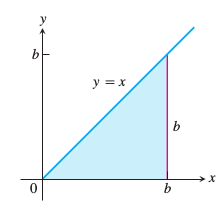
\includegraphics[width=10em]{ode_mattuck_94_int_01.png}

Her parca esit genislikte, $n$ tane var, $\Delta x = (b - 0) / n = b/n$,
parcalar $P = \left\{ 0, \frac{b}{n}, \frac{3b}{n}, ..., \frac{nb}{n}
\right\}$ her $c_k = \frac{kb}{n}$. O zaman 

$$ 
\sum_{k=1}^{n} f(c_k) \Delta x = \sum_{k=1}^{n} \frac{kb}{n} \cdot \frac{b}{n}
$$

$f(x) = x$ olduğu için doğal olarak $f(c_k)=c_k$ diyebildik. Devam edelim, 

$$ 
= \frac{kb^2}{n^2} = \frac{b^2}{n^2} \sum_{k=1}^{n} k
$$

$\sum_{k=1}^{n} k$ ilginç bir toplam, aslında 1'den n'ye kadar tüm
sayıları topla diyor, bu toplamın $\frac{n(n+1)}{2}$ olduğunu biliyoruz, 

$$ 
= \frac{b^2}{n^2} \frac{n(n+1)}{2}
$$

$$ 
\frac{b^2}{2} (1 + \frac{1}{n})
$$

$n \to \infty$ iken üstteki ifadenin $b^2/2$ limitine yaklaştığını
biliyoruz, yani

$$ 
\int_{0}^{b} x \ud x = \frac{b^2}{2}
$$


\newpage

Ekler

Entegralleri Nasıl Düşünelim

Calculus kitaplarında entegralleri anlatmak için çoğu zaman ``toplam''
kavramı on plana çıkarılır, mesela entegralin alttaki resimde $f(x)$
fonksiyonunun altında kalan ufak ufak dikdörtgenlerinin alanlarının
``toplamı'' olduğundan bahsedilir.

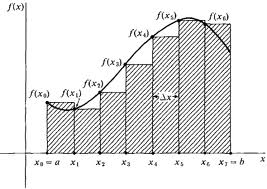
\includegraphics[height=4cm]{area.png}

Fakat bu tür bir anlatım bazen karışıklığa yol açabiliyor [2]. Daha iyi bir
anlatım entegralin ``değişen değerlerin çarpımı'' olduğudur. Alttaki
resimdeki dikdörtgeni düşünelim, 

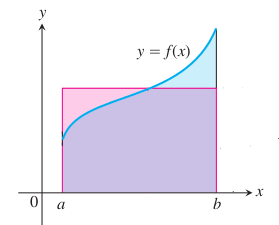
\includegraphics[height=4cm]{box.png}

ve diyelim ki bir dikdörtgen, entegralin hesapladığı alanı yaklaşıksal
olarak temsil ediyor. Dikdörtgen alanı nasıl hesaplanır? İki kenarının
çarpılmasıyla! Entegral de aslında böyle bir hesaptır, sadece kenarlardan
biri sabit değildir, ve sürekli değişmektedir. Bu tür bir anlayış birimleri
sonuca dahil etmek gerektiğinde ise yarar, mesela yatay ekşen zaman $t$
işe, ve dikey eksen hız $v(t)$ ise, katedilen mesafe, $v(t)$ nasıl bir
şekilde verilmiş olursa olsun,

$$ Mesafe = \int v(t) \ud t $$

formülüyle hesaplanacaktır. Eğer hız ve zaman sabit olsalar, mesela 5 ile 4
gibi, o zaman hesap son derece basit olacaktı, 3 x 4 = 12 ile sonucu
bulacaktık. 

Tabii ki çarpmak ile toplamak arasında yakın bağlantılar var, mesela 3 x
4'u şu şekilde resmedelim

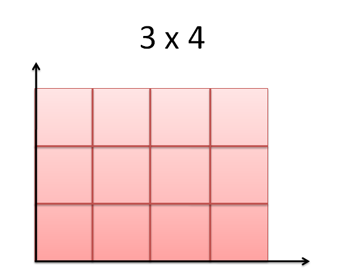
\includegraphics[height=4cm]{calc_multi_app_04.png}

Burada, evet, 3 değerini dört kere birbiriyle topluyoruz, 3 + 3 + 3 + 3 =
12 ve bu durum 3 x 4 ile aynı sonucu veriyor. Fakat 3'lerin toplamı, eğri
altındaki alan zihniyetini daha ilerletmeden azıcık farklı bir durumu
düşünelim. 

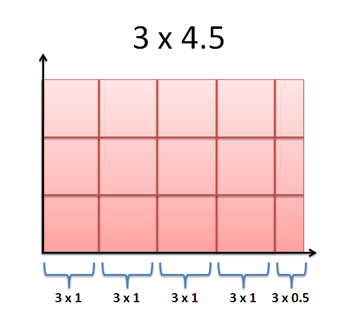
\includegraphics[height=4cm]{calc_multi_app_09.png}

Bu durumda dikey eksendeki kolonlara bir ek yaptık, ama bu ekin genişliği
tam bir kolon değil, yarım bir kolon. Bu durumda alan hesabını sadece dikey
kolonların toplanması olarak yapsakdik 3'u beş kere toplamamız gerekirdi,
ve 15 elde ederdik, yanlış bir hesap yapmış olurduk.

Toplamın doğru olması için yatay ekşenin genişliğinin hesaba katılması
gerekir, 3*1 + 3*1 + 3*1 + 3*1 + 3*0.5 = 13.5. Ya da tüm genişliği tüm
yükseklik ile çarparız 3 * 4.5 = 13.5. 

Peki ilk örneğe dönersek, madem çarpımlardan bahsediyoruz, diyelim ki
$v(t) = 2t$ o zaman $t \cdot 2t$ diyemez miyiz? Bu da olmaz, çünkü $t\cdot 2t = 2t^2$ 
bize sadece tek bir $t$ anındaki bir hesabı veriyor. Biz verilen bir 
başlangıç ve bitiş noktaları arasındaki ``tüm $t$'ler üzerindeki'' 
katedilen mesafeyle ilgileniyoruz.  

Yani entegral denince aklımıza çarpım gelsin, $x,y$ eksenleri bağlamında,
$y$ eksenindeki $f(x)$'i $x$'i çarpıyoruz, bu çarpım $x$ için entegrale
$dx$ olarak yansıyor, $f(x)$ ise entegre edilen fonksiyon haline geliyor. 

Birimleri hesaba katarsak anlatılanlar biraz daha anlamlanır belki. Eğer
hız km / saat ise, zaman saat ise, sadece hızların toplamı mesafe birimini
km / saat yapar, bu yanlış olur. Ama çarpım olarak düşünürsek km / saat *
saat = km sonucunu verir ki bu mesafenin birimidir. 

Ortalama mı, Toplam mı?

Diğer yandan bazen bir aralıkta bir fonksiyonun entegrali alındığında onun
``ortalamasından'' da bahsedildiğinin görebiliriz. Peki bir entegral bir
toplam midir (ya da akıllı çarpım) yoksa bir ortalama mı? Aslında bu iki
kavram arasında fazla bir fark yok; sonuçta 10 tane sayının toplamı ile
averajı arasında 1/10 sabiti ile çarpım haricinde bir fark yok [3]. 

Kaynaklar

[1] Thomas, {\em Thomas Calculus 11th Edition}

[2] Better Explained, {\em A Calculus Analogy: Integrals as  Multiplication},
    \url{http://betterexplained.com/articles/a-calculus-analogy-integrals-as-multiplication/}

[3] Quora, \url{https://www.quora.com/Is-an-integral-more-analogous-to-a-sum-or-to-an-average}

\end{document}
